%% Run with the following three lines uncommented for article pdf and comment for presentation pdf
%\documentclass[a4paper]{article}
%\usepackage{beamerarticle}
%\mode<article>{\usepackage{fullpage}}
%%

%% Run with the following line uncommented for presentation pdf and commented for article pdf
\documentclass[ignorenonframetext]{beamer}
%\documentclass[ignorenonframetext,draft]{beamer}
\setbeamertemplate{navigation symbols}{}
%%

\usepackage{ esint } % for multi-dimensional integrals
% \usepackage{movie15}
\usepackage{hyperref}
\usepackage{pgf}
\usepackage{subfigure}
% \usepackage{movie15}
\mode<presentation>
%{
%\usetheme{madrid}
%\usetheme{frankfurt}
    \usetheme{Copenhagen}
\useoutertheme{infolines} % this makes only immediate navigation at top of slide
%\setfootline{\insertshortinstitute, \insertshortdate
%\hfill slide \insertframenumber/\inserttotalframenumber}
%}
\setbeamertemplate{headline}{}

\title[SciPy 2014]{Perceptions of matplotlib colormaps}

\author{Kristen M. Thyng}
\date{July 10, 2014}
\institute[Texas A\&M]{Texas A\&M University}
    
% In case you want to use a logo (e.g. in png format): 
% \pgfdeclareimage[height=1.0cm]{university-logo}{figures/logo_tamu} 
% \logo{\pgfuseimage{university-logo}}

% \input{../../LatexFiles/macros}

% % Extra slides don't contribute to slide number at bottom right
% \input{appendixnumberbeamer.sty}

\AtBeginSection[]
{
    \begin{frame}
        \frametitle{Outline}
        \tableofcontents[currentsection]
    \end{frame}
}

\begin{document}
\begin{frame}
    \titlepage
\end{frame}


% \begin{frame}
%   \frametitle{Outline}
%   \tableofcontents
% \end{frame}


%%%  %%%

\section{}

\begin{frame}[t]\frametitle{CIELAB Color Model}
    \begin{figure}[htbp]
        \centering
        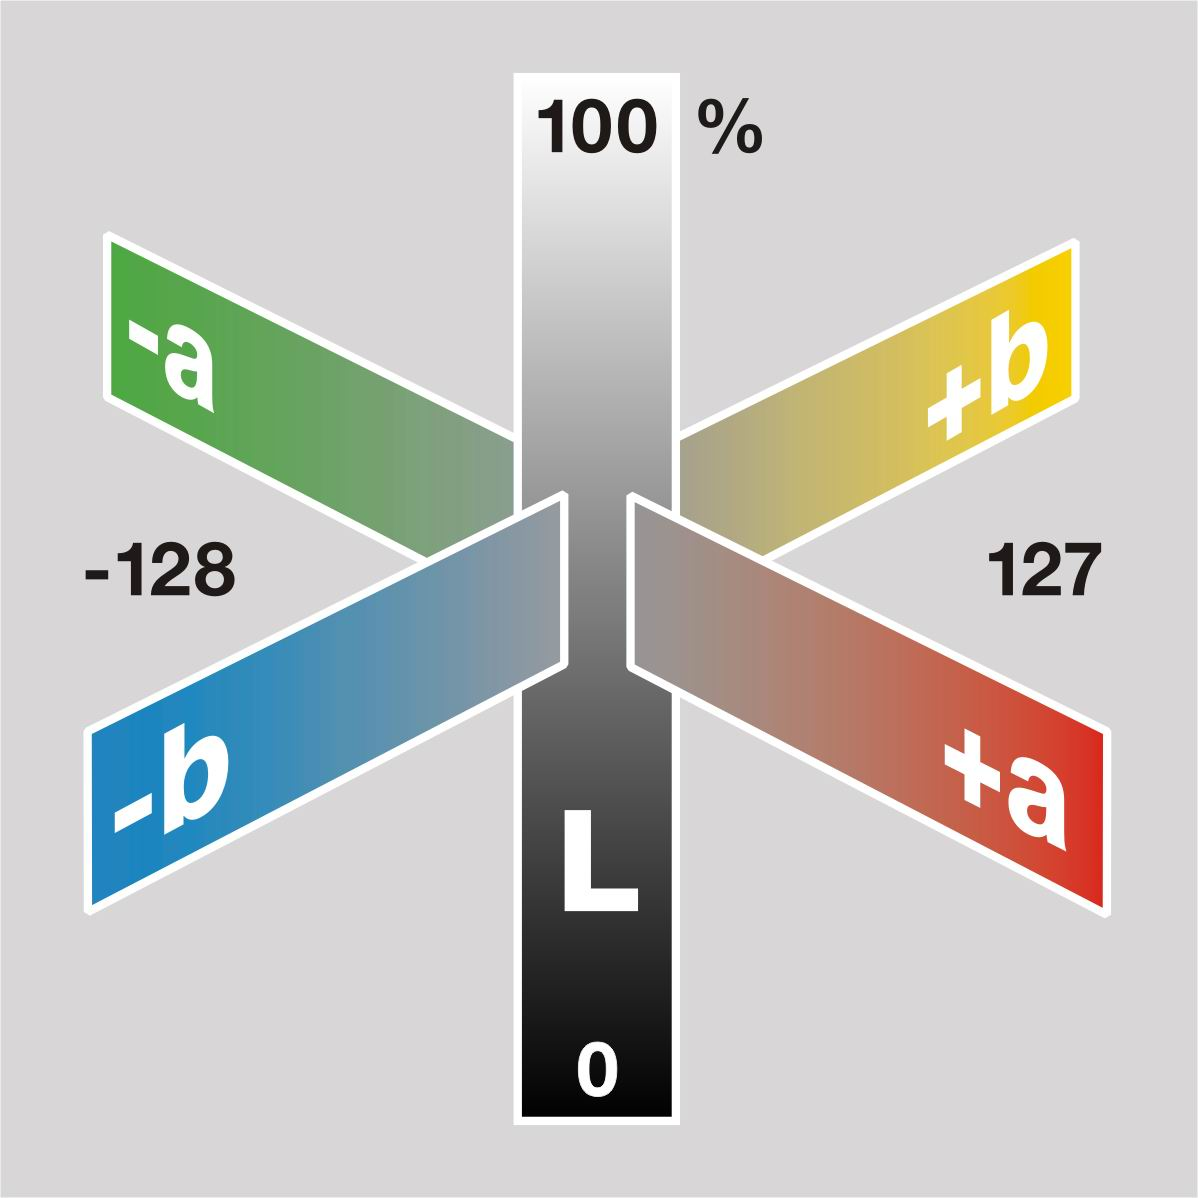
\includegraphics[width=0.55\textwidth]{figures/Cielab.jpg}
    \end{figure}
    \tiny{http://eschicleypega.blogspot.com}
\end{frame}

\begin{frame}[t]\frametitle{Lightness of matplotlib Colormaps}
    \begin{figure}[htbp]
        \centering
        \only<1>{
        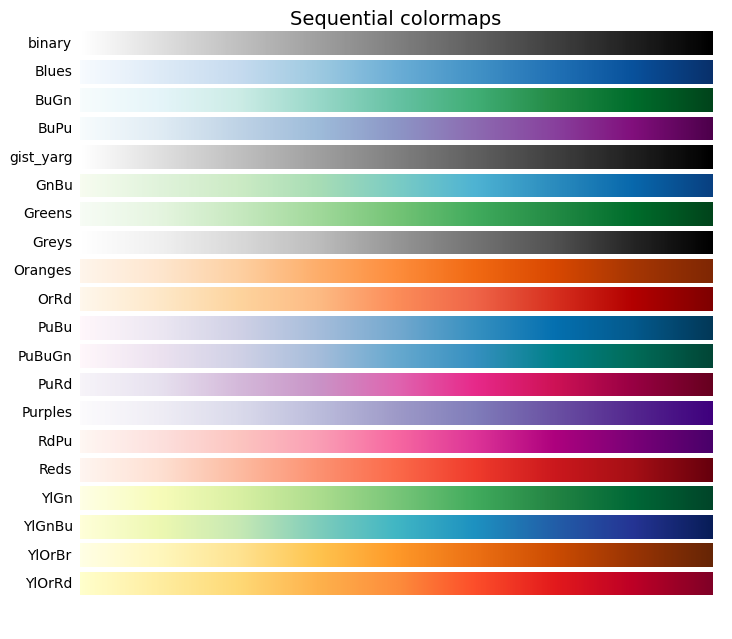
\includegraphics[width=0.45\textwidth]{figures/seq}
        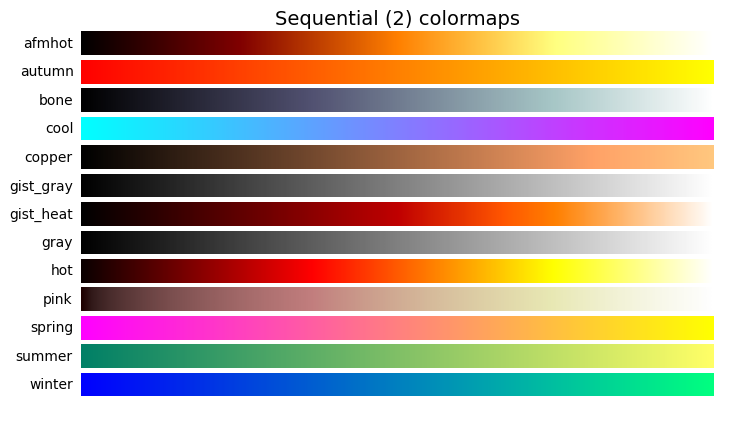
\includegraphics[width=0.45\textwidth]{figures/seq2}}
        \only<2>{
        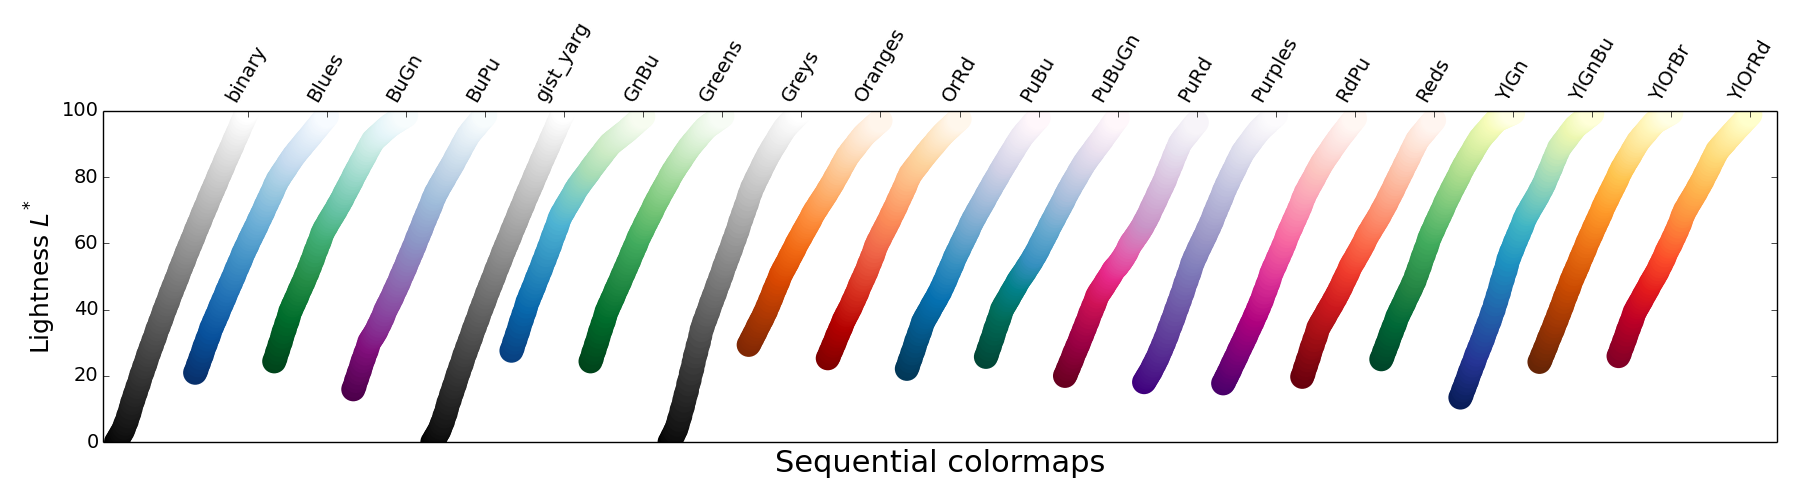
\includegraphics[width=\textwidth]{figures/lSequential} \\
        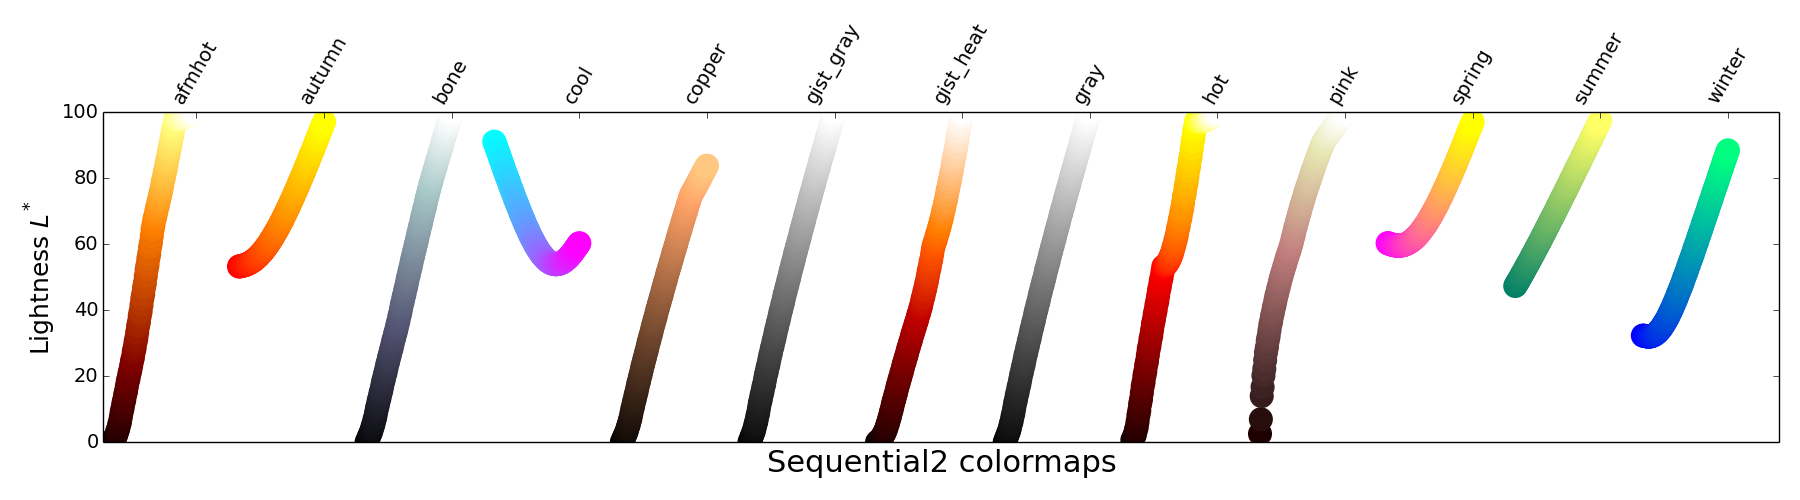
\includegraphics[width=\textwidth]{figures/lSequential2}
        }
    \end{figure}
    \only<1>{
    \vskip8ex
    \tiny{http://matplotlib.org/examples/color/colormaps\_reference.html}}
\end{frame}

\begin{frame}[t]\frametitle{Lightness of matplotlib Colormaps}
    \vskip-2ex
    \begin{figure}[htbp]
        \centering
        \only<1>{
        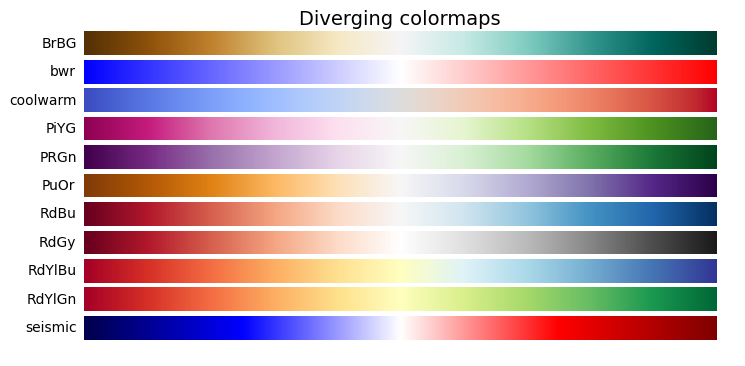
\includegraphics[width=0.45\textwidth]{figures/div}
        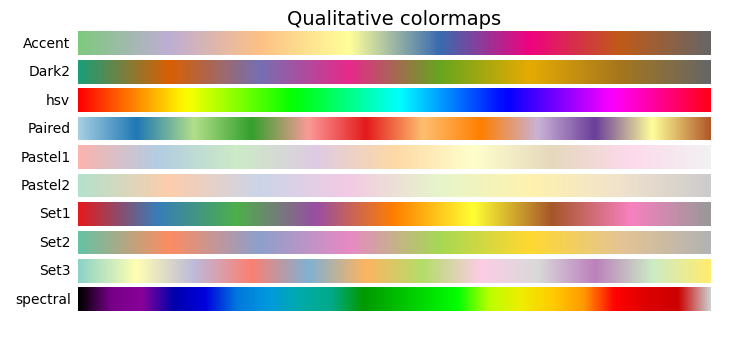
\includegraphics[width=0.45\textwidth]{figures/qual}\\
        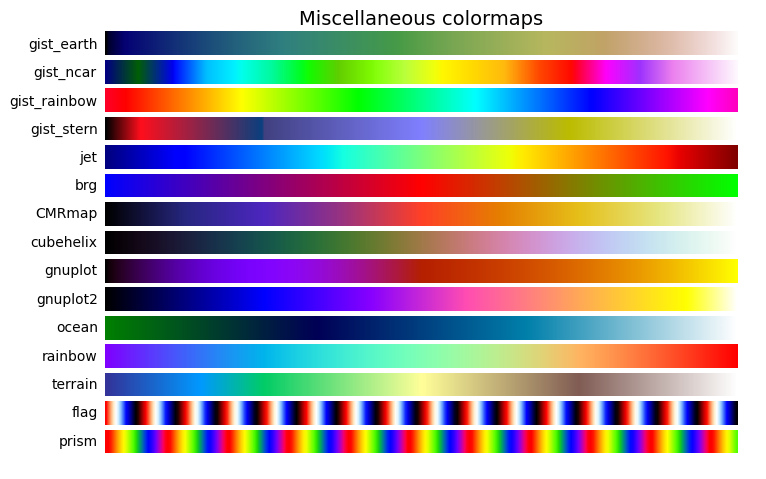
\includegraphics[width=0.45\textwidth]{figures/misc}}
        \only<2>{
        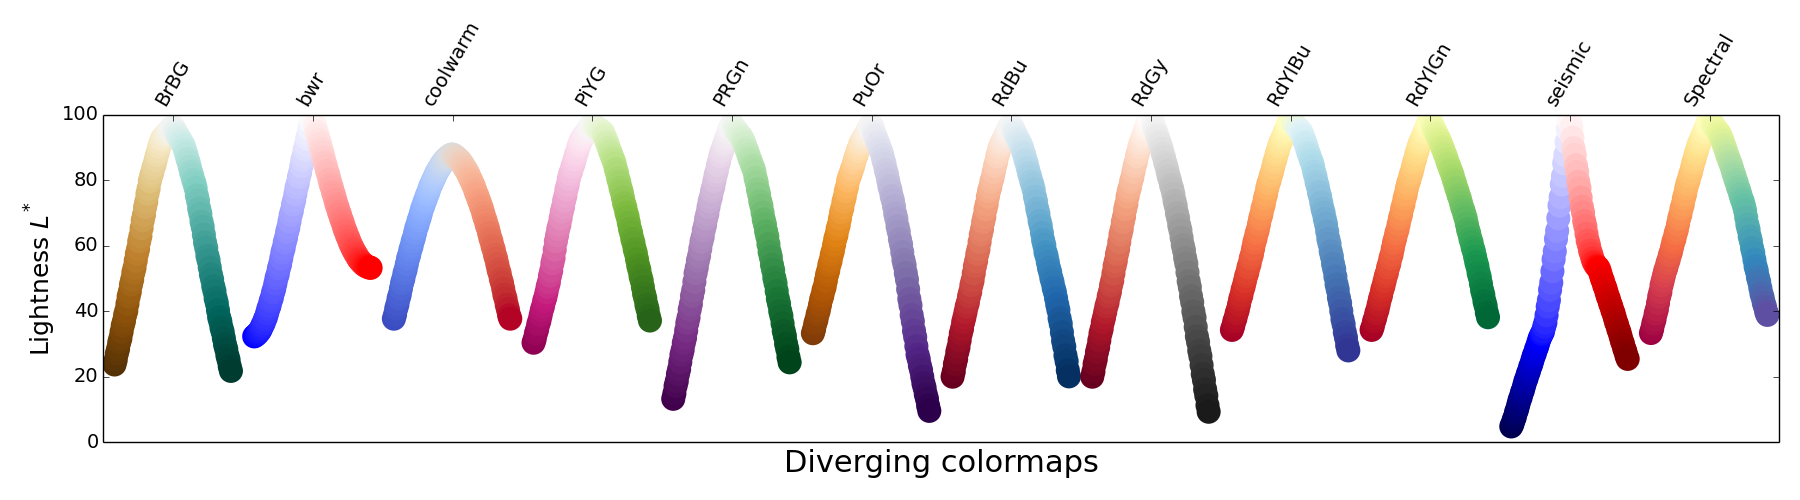
\includegraphics[width=0.8\textwidth]{figures/lDiverging} \\
        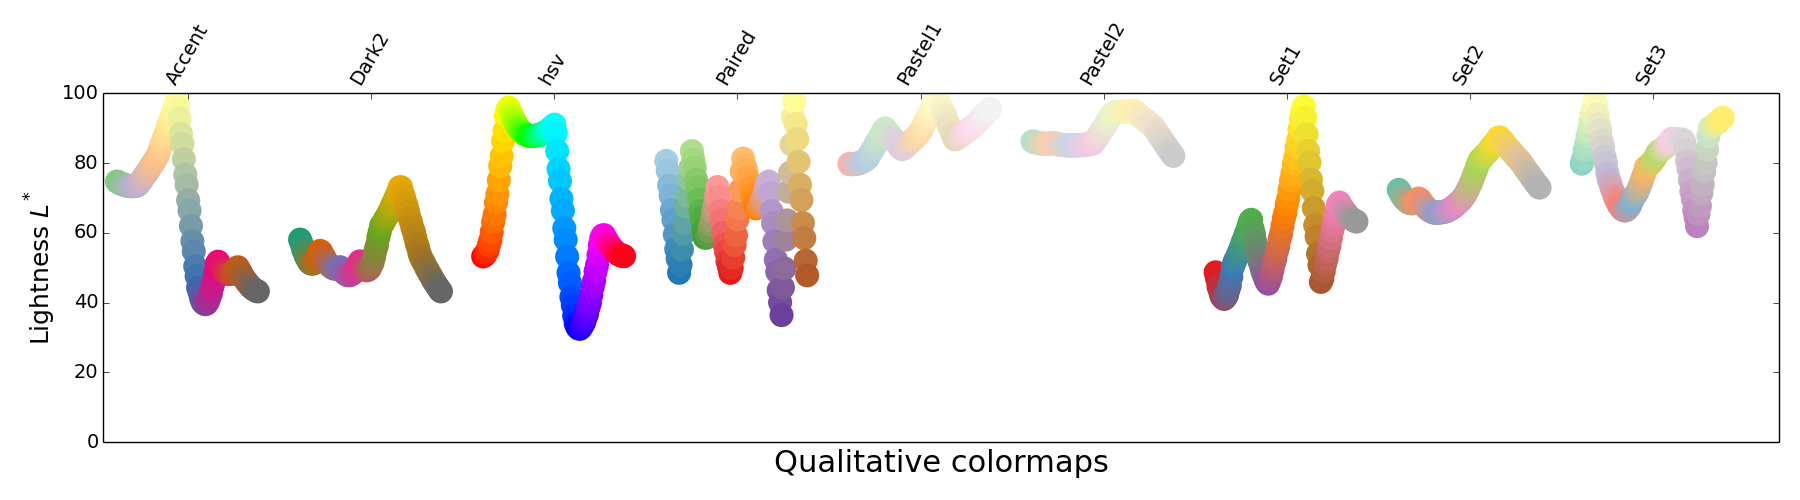
\includegraphics[width=0.8\textwidth]{figures/lQualitative} \\
        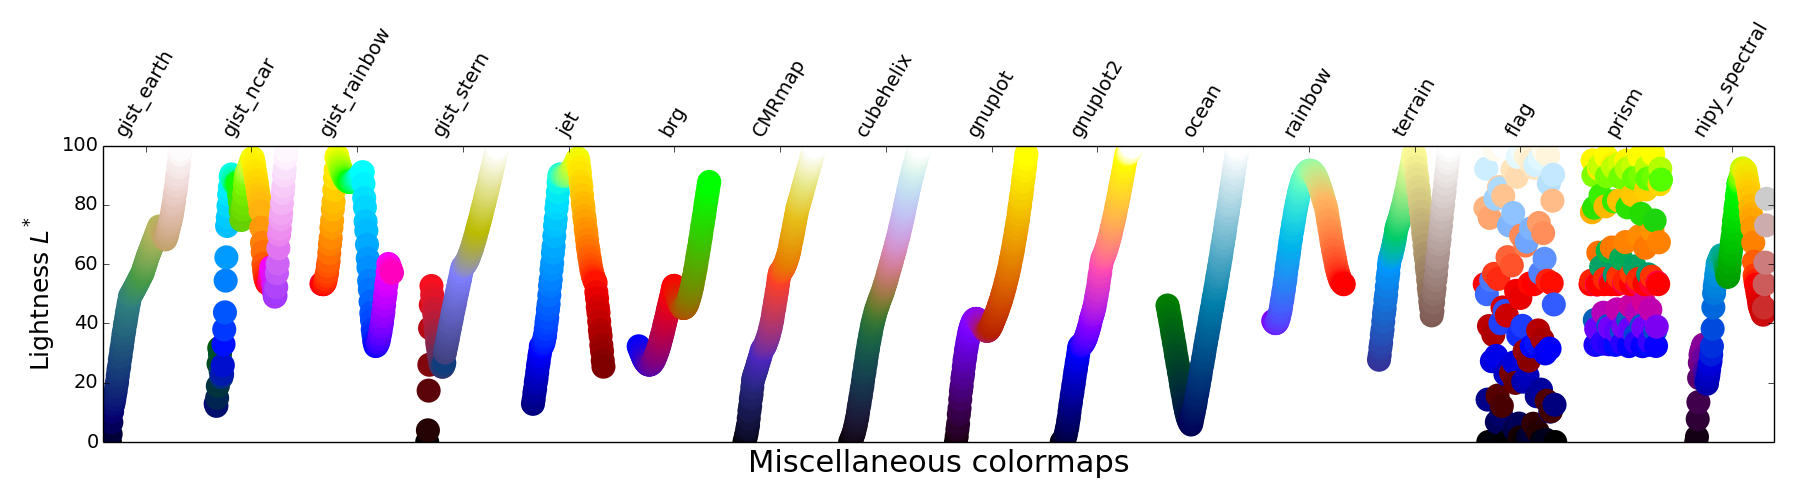
\includegraphics[width=0.8\textwidth]{figures/lMiscellaneous}
        }
    \end{figure}
    \only<1>{
    \tiny{http://matplotlib.org/examples/color/colormaps\_reference.html}}
\end{frame}

\begin{frame}[t]\frametitle{Perceived Lightness: Weber-Fechner Law (and Stevens)}
    \vskip-2ex
    \begin{figure}[htbp]
        \centering
        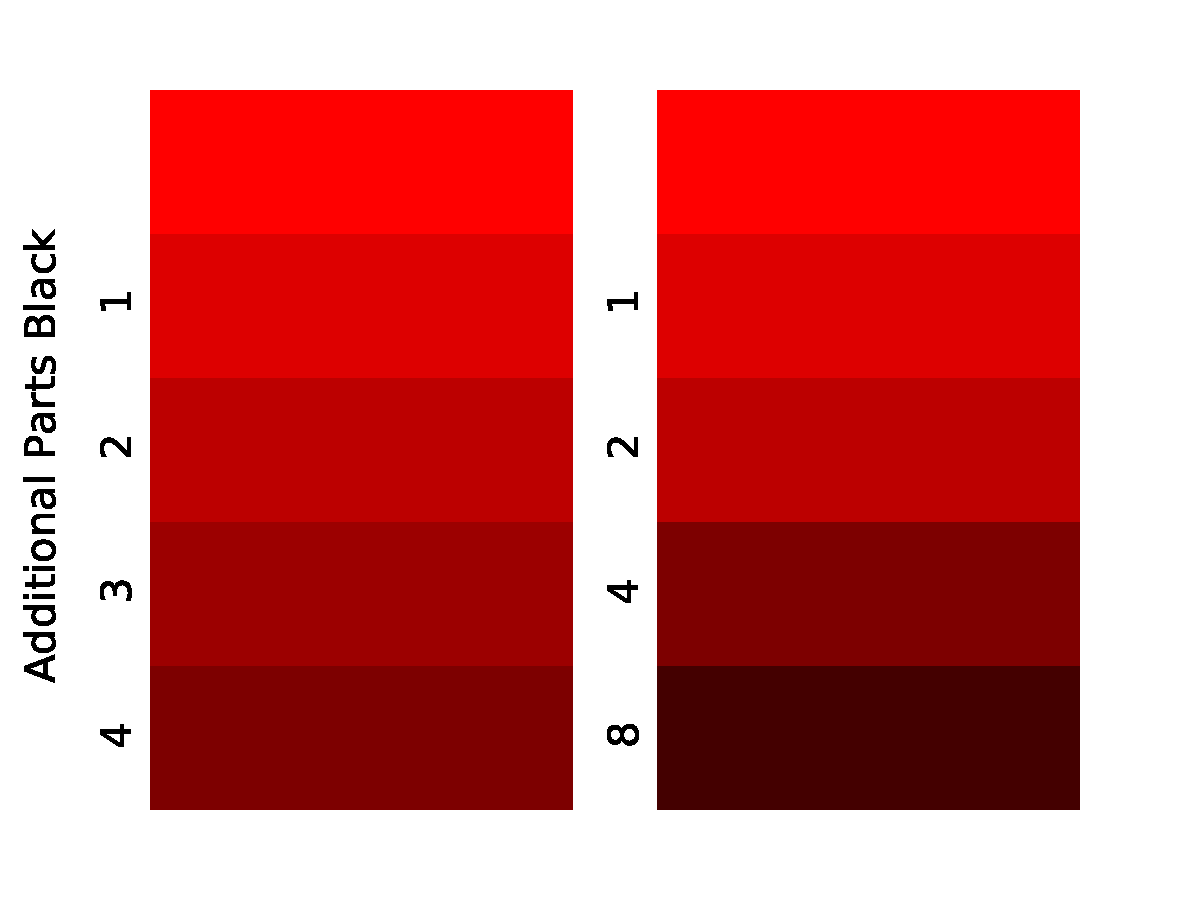
\includegraphics[width=0.8\textwidth]{figures/albers.pdf}
    \end{figure}
    \vskip-2ex
    \tiny{Albers, J. (1975). Interaction of color. Yale University Press.}
\end{frame}

\begin{frame}[t]\frametitle{Improvement to Binary Colormap?}
    \begin{figure}[htbp]
        \centering
        \only<1>{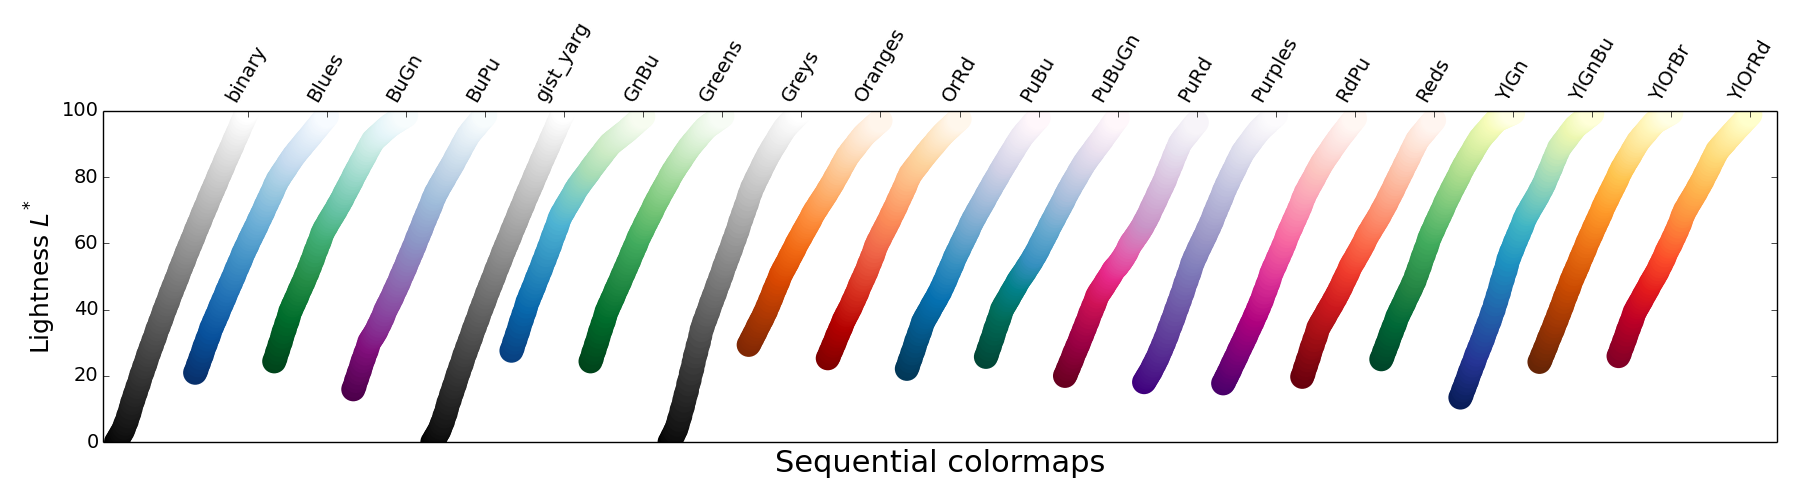
\includegraphics[width=\textwidth]{figures/lSequential}}
        \only<2>{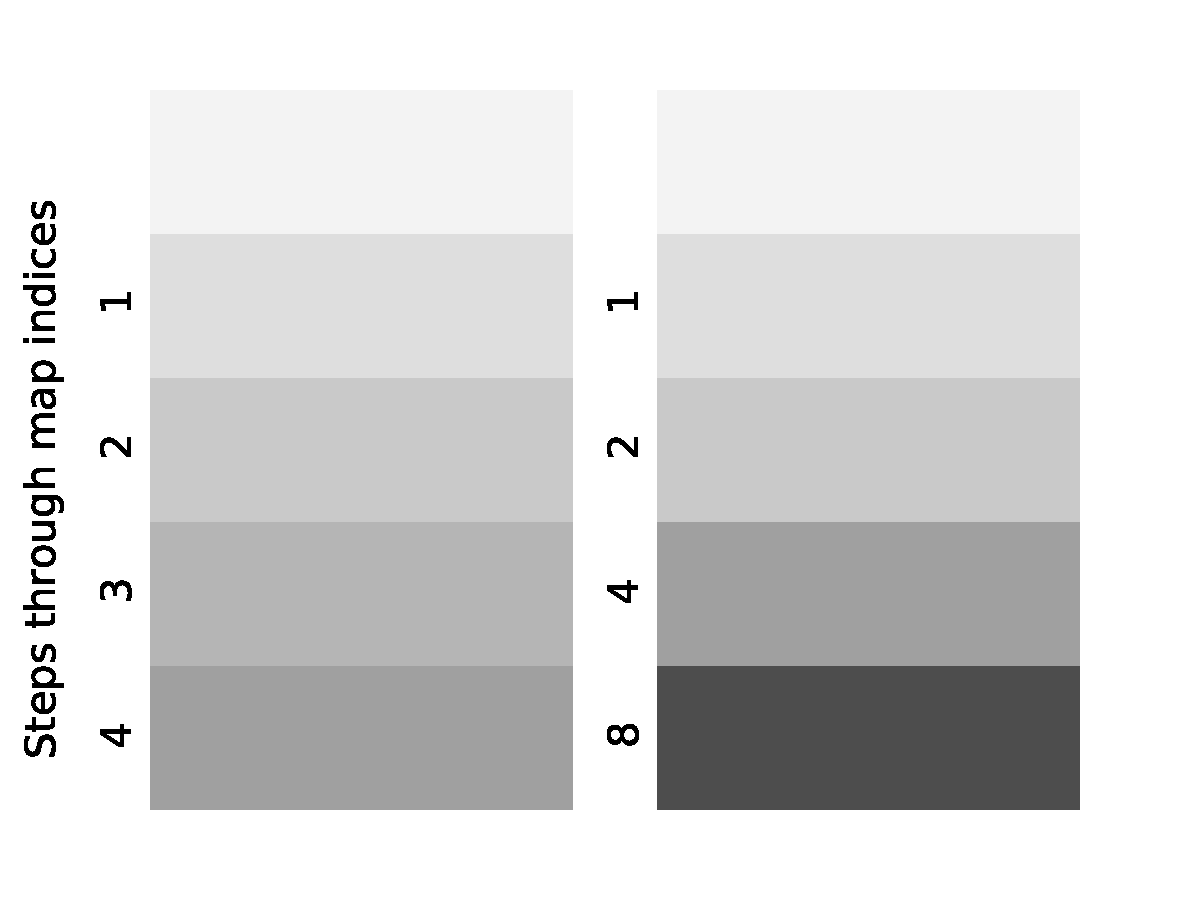
\includegraphics[width=0.8\textwidth]{figures/albers-bw}}
    \end{figure}
\end{frame}

\begin{frame}[t]\frametitle{Printing to Grayscale}
    \begin{itemize}
        \item {\Large Lots of ways to convert to grayscale}
        \item[]
        \item {\Large Gray = (Red * 0.2126 + Green * 0.7152 + Blue * 0.0722) (or similar$^*$)}
        \item[]
        \item {\Large Use luminance}
    \end{itemize}
    \vskip20ex
    {\tiny $^*$ http://www.tannerhelland.com/3643/grayscale-image-algorithm-vb6/}
\end{frame}

\begin{frame}[t]\frametitle{matplotlib Colormaps in Grey Scale}
    \begin{figure}[htbp]
        \centering
        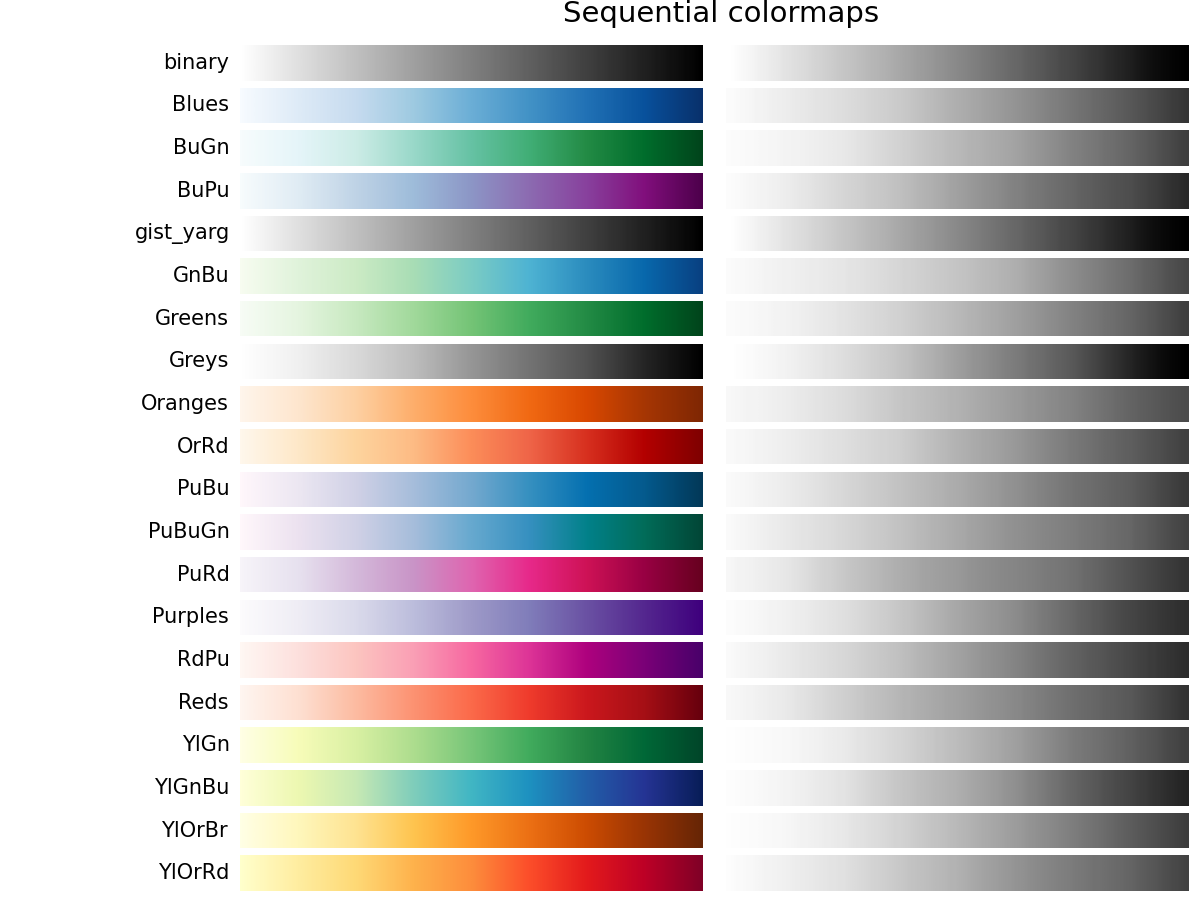
\includegraphics[width=0.7\textwidth]{figures/bwSequential}
    \end{figure}
\end{frame}
\begin{frame}[t,noframenumbering]\frametitle{matplotlib Colormaps in Grey Scale}
    \begin{figure}[htbp]
        \centering
        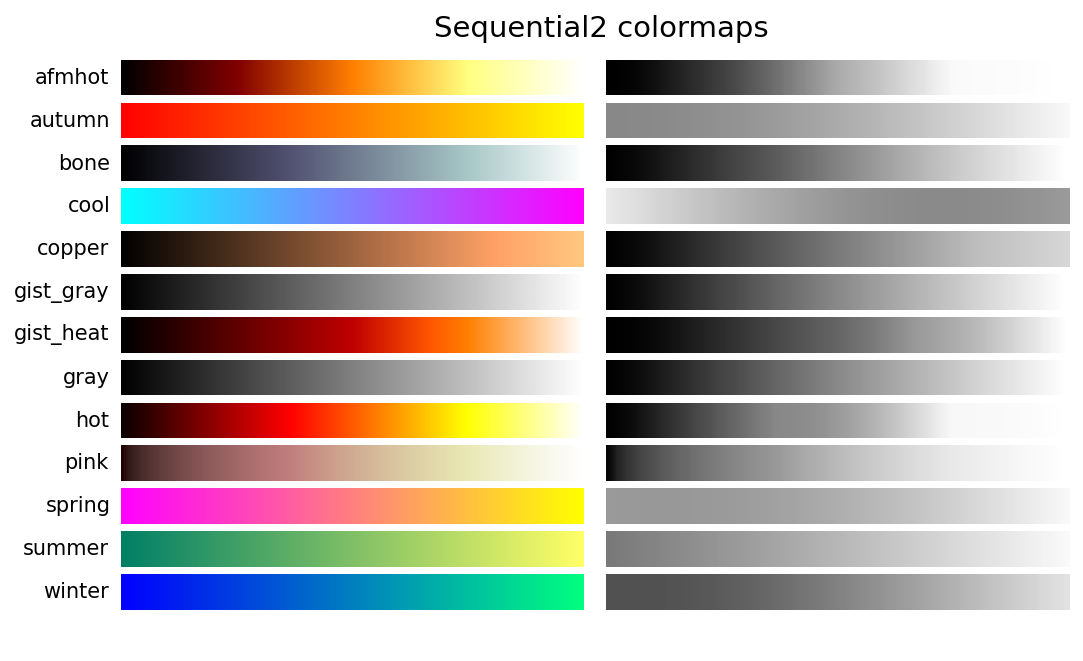
\includegraphics[width=\textwidth]{figures/bwSequential2}
    \end{figure}
\end{frame}
\begin{frame}[t,noframenumbering]\frametitle{matplotlib Colormaps in Grey Scale}
    \begin{figure}[htbp]
        \centering
        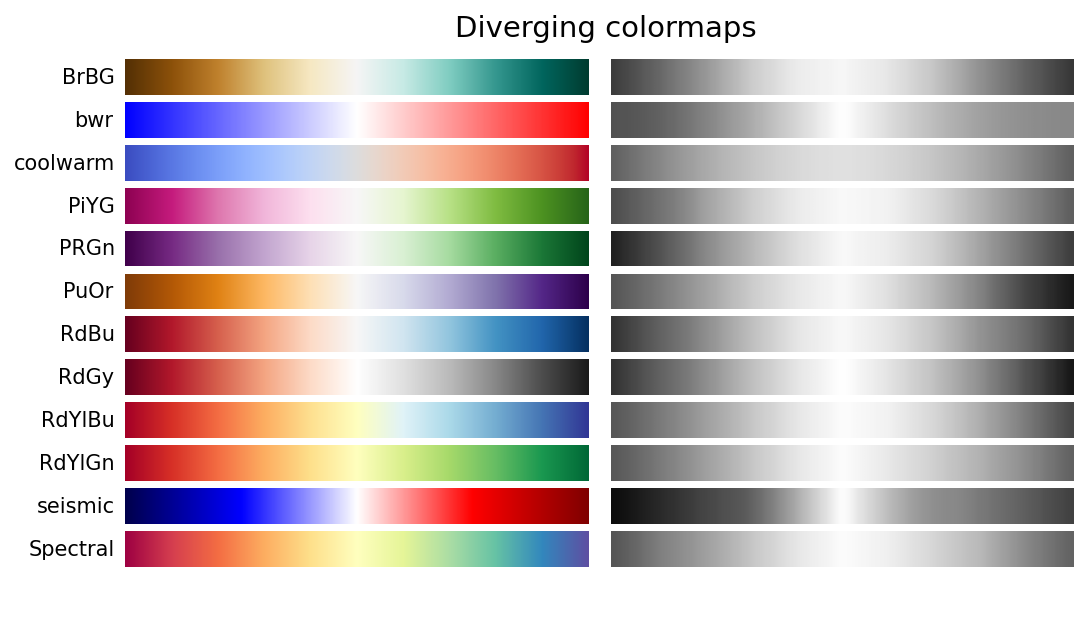
\includegraphics[width=\textwidth]{figures/bwDiverging}
    \end{figure}
\end{frame}
\begin{frame}[t,noframenumbering]\frametitle{matplotlib Colormaps in Grey Scale}
    \begin{figure}[htbp]
        \centering
        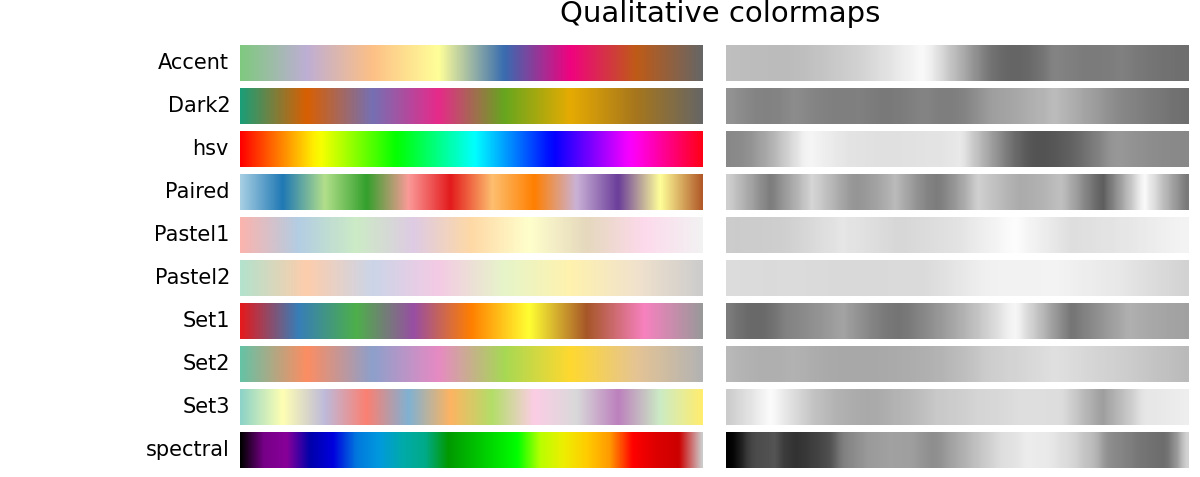
\includegraphics[width=\textwidth]{figures/bwQualitative}
    \end{figure}
\end{frame}
\begin{frame}[t,noframenumbering]\frametitle{matplotlib Colormaps in Grey Scale}
    \begin{figure}[htbp]
        \centering
        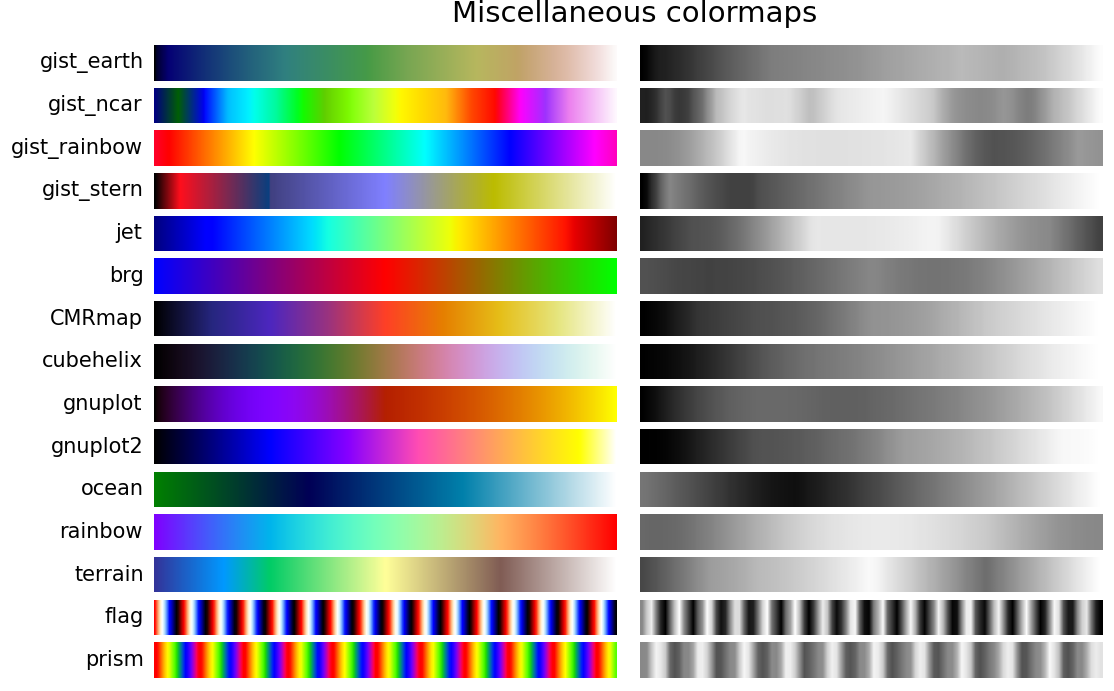
\includegraphics[width=\textwidth]{figures/bwMiscellaneous}
    \end{figure}
\end{frame}

\begin{frame}[t]\frametitle{Color Blindness}
    Protanopia (2\% male population, half mild form)
    \begin{figure}[htbp]
        \centering
        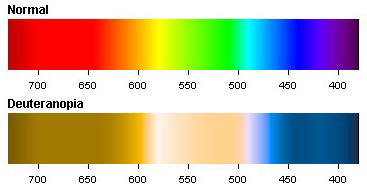
\includegraphics[width=0.43\textwidth]{figures/deuteranopia-color-spectrum}
    \end{figure}
    Deuteranopia (6\% male population, mostly mild form)
    \begin{figure}[htbp]
        \centering
        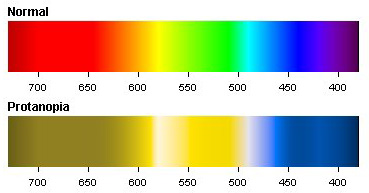
\includegraphics[width=0.43\textwidth]{figures/Protanopia-Color-Spectrum}
    \end{figure}
    \vskip-1ex
    \tiny{http://www.color-blindness.com}
\end{frame}
\begin{frame}[t]\frametitle{Color Blindness}
    \begin{figure}[htbp]
        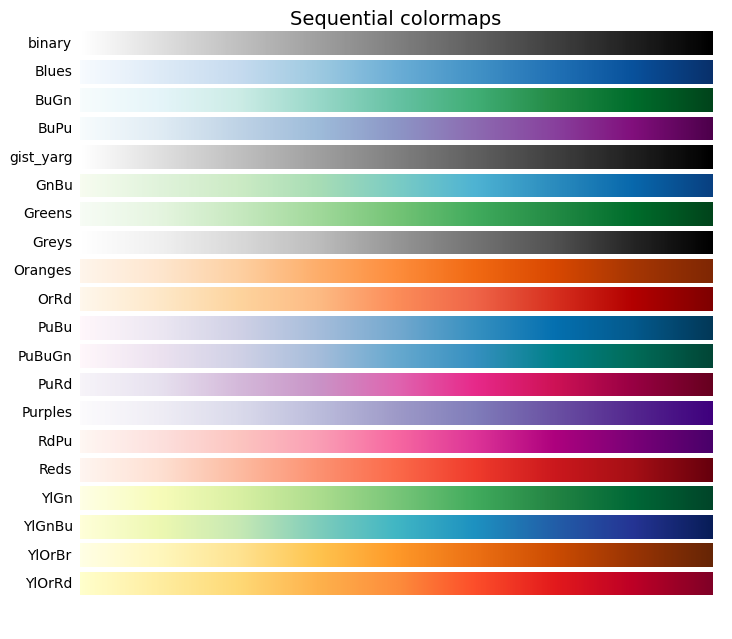
\includegraphics[width=0.49\textwidth]{figures/seq}
        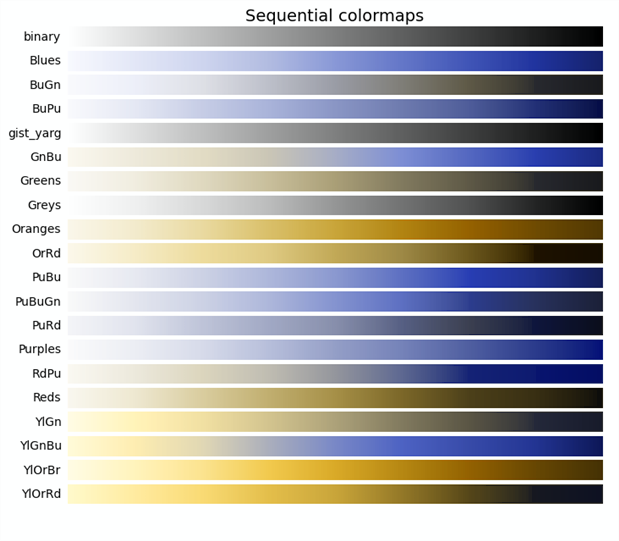
\includegraphics[width=0.49\textwidth]{figures/seq_deuteranopia}
    \end{figure}
    \vskip8ex
    \tiny{http://aspnetresources.com/tools/colorBlindness}
\end{frame}
\begin{frame}[t]\frametitle{Color Blindness}
    \begin{figure}[htbp]
        \centering
        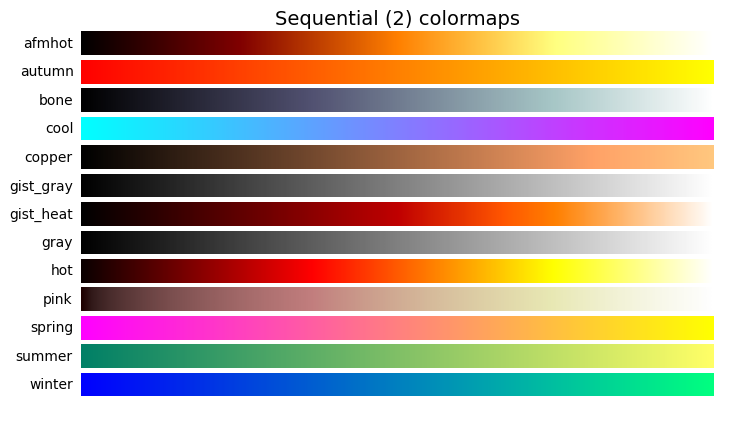
\includegraphics[width=0.49\textwidth]{figures/seq2}
        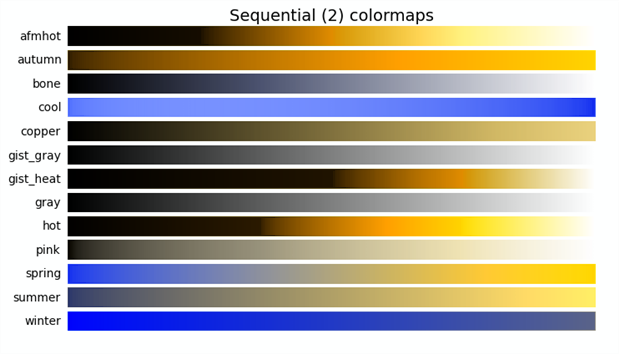
\includegraphics[width=0.49\textwidth]{figures/seq2_deuteranopia}
    \end{figure}
    \vskip18ex
    \tiny{http://aspnetresources.com/tools/colorBlindness}
\end{frame}
\begin{frame}[t]\frametitle{Color Blindness}
    \begin{figure}[htbp]
        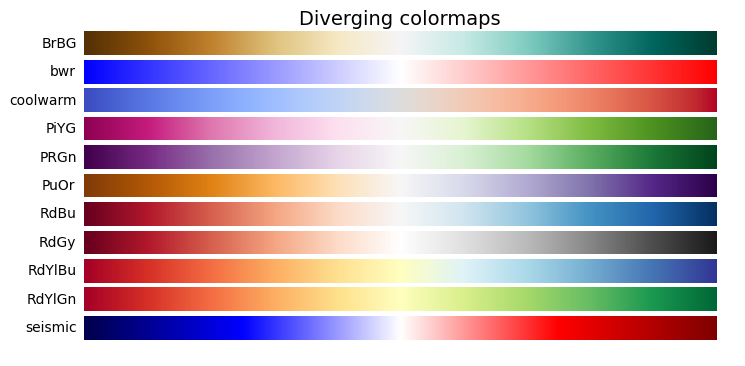
\includegraphics[width=0.49\textwidth]{figures/div}
        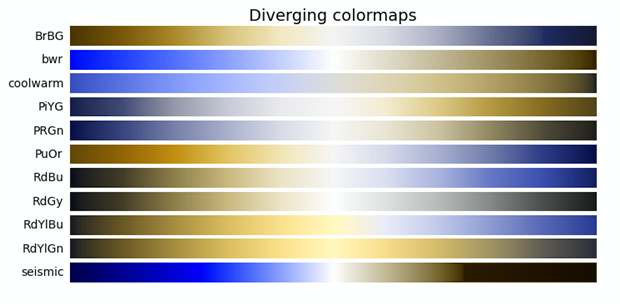
\includegraphics[width=0.49\textwidth]{figures/div_deuteranopia}
    \end{figure}
    \vskip22ex
    \tiny{http://aspnetresources.com/tools/colorBlindness}
\end{frame}
\begin{frame}[t]\frametitle{Color Blindness}
    \begin{figure}[htbp]
        \centering
        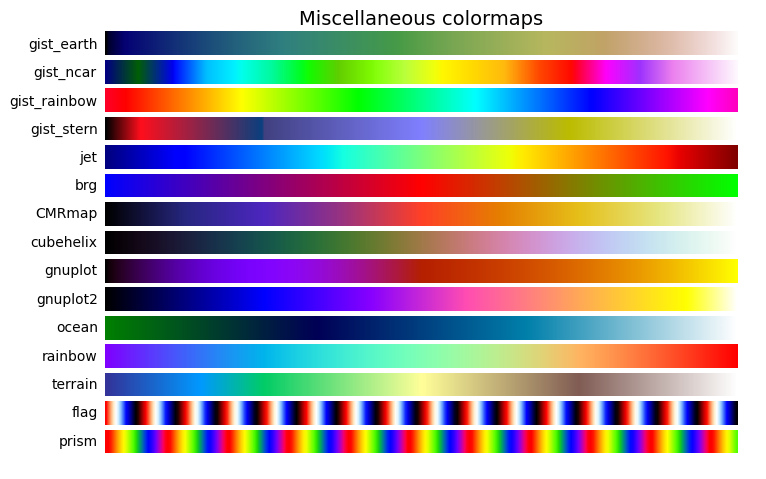
\includegraphics[width=0.49\textwidth]{figures/misc}
        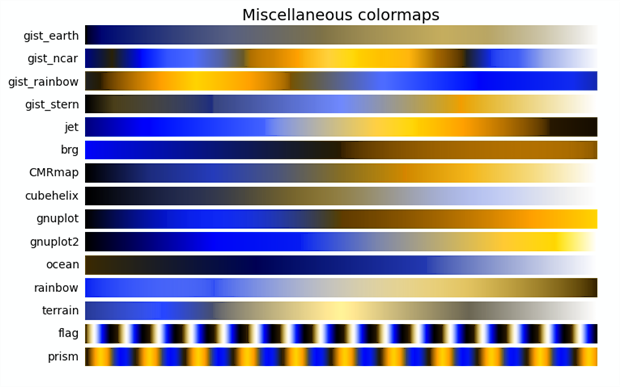
\includegraphics[width=0.49\textwidth]{figures/misc_deuteranopia}
    \end{figure}
    \vskip16ex
    \tiny{http://aspnetresources.com/tools/colorBlindness}
\end{frame}

\begin{frame}[c]\frametitle{Recommendations}
\begin{itemize}
    \item Best colormap depends on application, but for form information, perceptual colormaps are best
    \item[] ~
    \item Perceptual colormaps monotonically increase with lightness
    \item[] ~
    \item Not clear (to me) what functional relationship with L is best
    \item[] ~
    \item Many ways to convert to grayscale --- luminance is a good proxy to decide on a good map
    \item[] ~
    \item Most common color blindness problem is red-green --- try to avoid for reaching audiences most effectively
\end{itemize}
\end{frame}

\begin{frame}[c]\frametitle{Resources}
\begin{itemize}
    \item[] All around helpful information on colormaps: \\Matteo Niccoli: http://mycarta.wordpress.com/2012/05/29/the-rainbow-is-dead-long-live-the-rainbow-series-outline/
    \item[] ~
    \item[] Comparison of 7 methods of converting to grayscale: http://www.tannerhelland.com/3643/grayscale-image-algorithm-vb6/
    \item[] ~
    \item[] Color blindness: http://www.color-blindness.com
    \item[] ~
    \item[] Link to slides:  \url{https://github.com/dmcdougall/scipy14-colormaps}
\end{itemize}
\end{frame}

\end{document}
